% ============================================================================
% OLG Models with Deep Equilibrium Nets
%
% Organization (Turin-style, analytic-model first):
%   Part 0   Title + roadmap                        (2)
%   Part I   Motivation + what is OLG?              (3)
%   Part II  Analytic 6-agent Krueger-Kubler (2004)  (14)
%            setup -> hh -> firms -> equilibrium ->
%            FOCs -> cost -> FREE -> architecture ->
%            training -> exercise -> validation
%   Part III Benchmark (AGS 2022 leading example)    (5)
%            slides only; the working code is the
%            upstream DeepEquilibriumNets repository
%            same 9-step skeleton, applied to
%            the 56-cohort two-asset model that
%            the upstream DeepEquilibriumNets repo implements
%   Part IV  Wrap-up + references                    (2)
% ============================================================================

\documentclass[aspectratio=169,11pt]{beamer}

% ---------- Theme and colors ----------
\usecolortheme{dove}
\setbeamertemplate{navigation symbols}{}
\setbeamertemplate{footline}{%
  \hfill\usebeamerfont{page number in head/foot}%
  \usebeamercolor[fg]{normal text}%
  \insertframenumber\,/\,\inserttotalframenumber\kern1em\vskip4pt}
\setbeamerfont{frametitle}{size=\huge}

% ---------- Packages ----------
\usepackage[utf8]{inputenc}
\usepackage[T1]{fontenc}
\usepackage{lmodern}
\usepackage{amsmath,amssymb,amsfonts}
\usepackage{bm}
\usepackage{graphicx}
\usepackage{tikz}
\usetikzlibrary{shapes,arrows.meta,positioning,calc,fit,backgrounds,patterns,decorations.pathreplacing}
\usepackage{pgfplots}
\pgfplotsset{compat=1.18}
\usepackage{booktabs}
\usepackage{hyperref}
\usepackage{xcolor}

% ---------- Custom colors ----------
\definecolor{uzhblue}{rgb}{0,0,0.5}
\definecolor{uzhgreylight}{RGB}{236,238,241}
\definecolor{uzhgreydark}{RGB}{81,86,94}
\definecolor{harvardcrimson}{RGB}{153,0,0}
\definecolor{unil@blue}{RGB}{0,140,204}
\definecolor{unil@black}{RGB}{35,31,32}
\definecolor{darkgreen}{RGB}{0,100,0}
\definecolor{darkred}{RGB}{139,0,0}
\definecolor{softblue}{RGB}{70,130,180}
\definecolor{softorange}{RGB}{230,159,0}
\definecolor{softgreen}{RGB}{0,158,115}

% ---------- Set beamer colors ----------
\setbeamercolor{frametitle}{bg=uzhgreylight, fg=uzhblue}
\setbeamercolor{title}{fg=uzhblue}
\setbeamercolor{structure}{fg=uzhblue}
\setbeamercolor{block title}{bg=unil@blue, fg=white}
\setbeamercolor{block body}{bg=uzhgreylight}
\setbeamercolor{block title alerted}{bg=darkred,fg=white}
\setbeamercolor{block body alerted}{bg=red!5}
\setbeamercolor{block title example}{bg=darkgreen,fg=white}
\setbeamercolor{block body example}{bg=green!5}
\setbeamercolor{item}{fg=unil@black}
\setbeamercolor{normal text}{fg=unil@black}

% ---------- Emphasis and hyperlinks ----------
\newcommand{\emphc}[1]{\textcolor{harvardcrimson}{#1}}
\hypersetup{colorlinks,linkcolor=harvardcrimson,urlcolor=harvardcrimson}

% ---------- Math shortcuts ----------
\newcommand{\R}{\mathbb{R}}
\newcommand{\E}[1]{\mathbb{E}\!\left[#1\right]}
\newcommand{\N}{\mathcal{N}}
\newcommand{\Loss}{\mathcal{L}}
\newcommand{\st}{\text{s.t.}\ }
\newcommand{\ubr}[2]{\underbrace{#1}_{\text{\scriptsize #2}}}

% ---------- Title ----------
\title[OLG -- Padova 2026]%
{Deep Learning for Solving Dynamic Models}
\subtitle{Session 4: Overlapping generations with DEQNs}
\author{Simon Scheidegger}
\institute[HEC Lausanne]{HEC, University of Lausanne}
\date{University of Padova\\September 23, 2026}

\begin{document}

% =====================================================================
% Part 0 -- Title + roadmap
% =====================================================================
{\setbeamercolor{background canvas}{bg=uzhgreylight}
\begin{frame}
\titlepage
\vspace{-0.4cm}
\begin{center}
{\footnotesize Based on Azinovic, Gaegauf \& Scheidegger (2022, \emph{IER} 63(4), 1471--1525) and Krueger \& K\"ubler (2004, \emph{JEDC}).}
\end{center}
\end{frame}
}

\begin{frame}{Roadmap}
\small
\begin{block}{Part I: What is an OLG model?}
Why overlapping generations; the cohort structure; the DEQN recipe in one line.
\end{block}
\begin{block}{Part I\textonehalf: The simplest OLG, two periods (Diamond, 1965)}
One decision, one Euler equation, one closed form. Notebook \texttt{04\_00}.
\end{block}
\begin{block}{Part II: The analytic six-agent model (Krueger \& K\"ubler, 2004)}
Euler equation and closed form derived; recursive equilibrium; cost function; network; validation. Notebook \texttt{04\_01}.
\end{block}
\begin{block}{Part III: The 56-cohort benchmark of Azinovic, Gaegauf \& Scheidegger (2022)}
CRRA, hump-shaped labor, two assets, two constraints, persistent shocks. Slides only: the working code,
with the paper's trained weights, is the \texttt{DeepEquilibriumNets} repository.
\end{block}
\end{frame}

% --- Learning objectives ---
\begin{frame}{Learning objectives}
\textbf{By the end of this lecture you should be able to:}
\begin{itemize}
  \item Derive the Euler equation and the closed-form savings rate of a log-utility OLG economy, and say precisely which two assumptions make the closed form possible
  \item Construct a finite-dimensional overlapping-generations equilibrium with cohort-specific savings and lifecycle heterogeneity
  \item Derive equilibrium conditions and build the mean-squared Euler-residual loss for a multi-cohort OLG model
  \item Implement the DEQN recipe: model specification, equilibrium definition, cost function, network training, and validation
  \item Validate a learned solution against the closed-form equilibrium in the analytic Krueger--K\"ubler model
  \item Read a research-scale benchmark (56 cohorts, two assets, two constraints, adjustment costs) as the same recipe with a larger $G$
\end{itemize}
\end{frame}



% =====================================================================
% Part I -- Motivation + what is OLG?
% =====================================================================

\section{Part I: What is an OLG model?}

\begin{frame}{Why Overlapping Generations?}
\footnotesize
\begin{block}{The economic content}
\vspace{-3pt}\begin{itemize}\itemsep2pt
    \item \emphc{Lifecycle:} agents are born, work, save, retire, die.  A representative infinitely-lived household cannot speak to pensions, retirement, inheritance, or cohort-specific shocks.
    \item \emphc{Demographics:} at any $t$, many cohorts coexist, each with its own asset holdings and labor income.
    \item \emphc{Finite asset distribution:} with $A$ cohorts, the cross-sectional wealth distribution is an $A$-vector, not an infinite-dimensional object.  \emphc{Suited to DEQNs:} the state stays finite-dimensional with realistic heterogeneity.
\end{itemize}
\end{block}
\vspace{-3pt}
\begin{block}{Two canonical versions we solve today}
\vspace{-3pt}\begin{enumerate}\itemsep1pt
    \item $A=6$ analytic model (Krueger \& K\"ubler, 2004): closed form $\Rightarrow$ ground-truth validation.
    \item $A=56$ leading-example benchmark (Azinovic, Gaegauf \& Scheidegger, 2022, \S 3): research-scale, no closed form.
\end{enumerate}
\end{block}
\end{frame}


\begin{frame}{OLG Structure: Overlapping Cohorts}
\centering
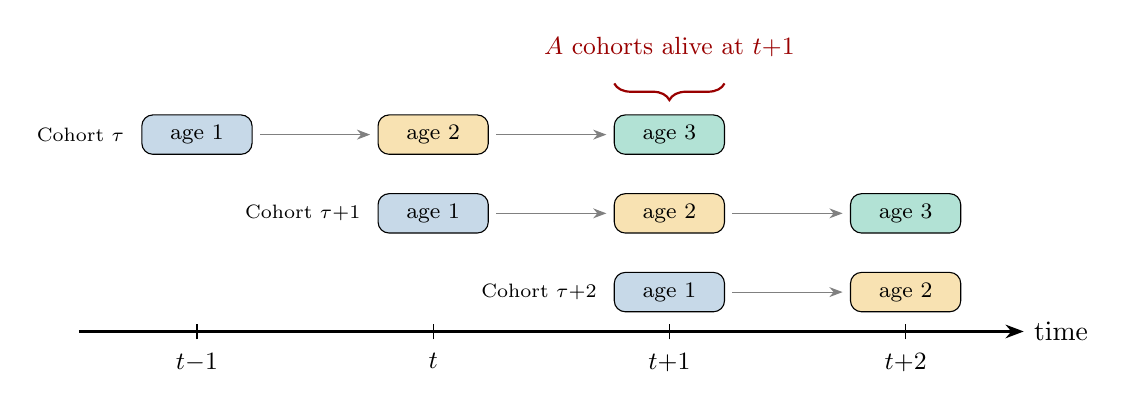
\begin{tikzpicture}[
    agent/.style={draw, rounded corners, minimum width=1.4cm, minimum height=0.5cm, font=\footnotesize},
    young/.style={agent, fill=softblue!30},
    mid/.style={agent, fill=softorange!30},
    old/.style={agent, fill=softgreen!30},
    >=Stealth
]
% Time axis
\draw[->, thick] (-0.5,0) -- (11.5,0) node[right] {time};
\foreach \t/\lab in {1/t{-}1, 4/t, 7/t{+}1, 10/t{+}2} {
    \draw (\t, -0.1) -- (\t, 0.1);
    \node[below] at (\t, -0.15) {\small $\lab$};
}

% Cohort 1 (born t-1)
\node[young] at (1, 2.5) {age 1};
\node[mid]   at (4, 2.5) {age 2};
\node[old]   at (7, 2.5) {age 3};
\draw[->, gray] (1.8, 2.5) -- (3.2, 2.5);
\draw[->, gray] (4.8, 2.5) -- (6.2, 2.5);
\node[left, font=\scriptsize] at (0.2, 2.5) {Cohort $\tau$};

% Cohort 2 (born t)
\node[young] at (4, 1.5) {age 1};
\node[mid]   at (7, 1.5) {age 2};
\node[old]   at (10, 1.5) {age 3};
\draw[->, gray] (4.8, 1.5) -- (6.2, 1.5);
\draw[->, gray] (7.8, 1.5) -- (9.2, 1.5);
\node[left, font=\scriptsize] at (3.2, 1.5) {Cohort $\tau{+}1$};

% Cohort 3 (born t+1)
\node[young] at (7, 0.5) {age 1};
\node[mid]   at (10, 0.5) {age 2};
\draw[->, gray] (7.8, 0.5) -- (9.2, 0.5);
\node[left, font=\scriptsize] at (6.2, 0.5) {Cohort $\tau{+}2$};

% Brace marking the t+1 column, placed above the diagram so it never
% crosses the inter-cohort transition arrows.
\draw[decorate, decoration={brace, amplitude=6pt, mirror}, thick, harvardcrimson]
    (6.3, 3.15) -- (7.7, 3.15)
    node[midway, above=6pt, font=\small, text=harvardcrimson]
    {$A$ cohorts alive at $t{+}1$};
\end{tikzpicture}

\vspace{0.3em}
At each period $t$ we have $A$ coexisting cohorts.  A newborn enters (age 1); the oldest dies (age $A$).\\
\emphc{Key observation:} the number of types is finite ($A$), so the cross-sectional state is finite-dimensional.
\end{frame}


\begin{frame}{The DEQN Recipe}
\small
\begin{block}{From model to neural network (to be applied twice in today's lecture)}
\begin{enumerate}\itemsep2pt
    \item Write down the \emphc{economic model}: preferences, technology, constraints, shocks.
    \item Define the \emphc{equilibrium}: choices + prices that satisfy optimization + market clearing.
    \item Write the \emphc{equilibrium conditions} as a system $G(x, f(x)) = 0$.
    \item Replace $f$ by a \emphc{neural network} $\N_\theta$ and form the \emphc{cost function} $\Loss(\theta) = \frac{1}{|D|}\sum_j \|G(x_j, \N_\theta(x_j))\|^2$.
    \item Sample training states $D$, minimize $\Loss(\theta)$ by SGD.
\end{enumerate}
\end{block}

\begin{alertblock}{The only thing that depends on the model}
The \emphc{equilibrium conditions $G$}.  Everything else, the network, the SGD loop, the sampling method, is generic.  \emphc{So to solve a new model, write down its $G$.}
\end{alertblock}

\vspace{0.2em}
{\footnotesize Today: derive $G$ explicitly for both the analytic and the benchmark OLG models.}
\end{frame}


% =====================================================================
% Part I 1/2 -- The simplest OLG: Diamond (1965), two periods
% =====================================================================

\section{Part I\textonehalf: The simplest OLG, two periods}

\begin{frame}{Diamond (1965): Two Periods, One Decision}
\small
\begin{columns}[T]
\column{0.55\textwidth}
\textbf{Households.}  Live two periods.
\begin{itemize}\itemsep2pt
    \item \emphc{Young:} work (one unit), earn $w_t$; consume $c^y_t$, save $s_t$ in capital:
          $c^y_t + s_t = w_t$.
    \item \emphc{Old:} no labor; sell the capital, consume the proceeds: $c^o_{t+1} = r_{t+1}\,s_t$.
    \item Preferences $\ln c^y_t + \beta\,\mathbb{E}_t \ln c^o_{t+1}$, \; $\beta = 0.7$.
\end{itemize}

\vspace{0.3em}
\textbf{Firm.}  Same technology as later: $\eta(z)K^\alpha L^{1-\alpha} + (1-\delta(z))K$, $L=1$.
The old hold all the capital: $K_t = s_{t-1}$.
\[
r_t = \alpha\eta(z_t)K_t^{\alpha-1} + 1 - \delta(z_t),\quad w_t = (1-\alpha)\eta(z_t)K_t^{\alpha}.
\]

\column{0.42\textwidth}
\begin{block}{State}
$(z_t,\,k_t)$ with $k_t = K_t$ the capital the old carry in. Prices are functions of it.
\end{block}
\begin{block}{Shocks}
The same four i.i.d.\ states $(\eta,\delta)$ as in Part II, probability $\tfrac14$ each.
\end{block}
\vspace{0.3em}
{\footnotesize \emphc{Why start here.}  Session 2's Brock--Mirman model also had one Euler equation and a
closed form.  What is new is that \emph{two different households are alive at the same date}, so the
cross-section is part of the state.  Two cohorts is the smallest structure with that property.}
\end{columns}
\end{frame}


\begin{frame}{The Euler Equation, Derived and Solved}
\small
Substitute both budget constraints: the young choose $s$ to maximise
\[
\ln(w_t - s) \;+\; \beta\,\mathbb{E}_t \ln\bigl(r_{t+1}\,s\bigr).
\]
\textbf{Step 1.}  $\ln(r_{t+1}s) = \ln r_{t+1} + \ln s$: the return and the choice \emphc{separate}.

\textbf{Step 2.}  First-order condition:
\[
\frac{1}{w_t - s} \;=\; \beta\,\mathbb{E}_t\!\left[\frac{r_{t+1}}{r_{t+1}\,s}\right] \;=\; \frac{\beta}{s}
\qquad\Longrightarrow\qquad
\boxed{\;s_t = \frac{\beta}{1+\beta}\,w_t \;=\; 0.4118\,w_t\;}
\]

\vspace{0.3em}
\begin{block}{Two observations}
\vspace{-2pt}\begin{enumerate}\itemsep1pt
    \item The return cancels. Under log utility the savings \emph{rate} does not depend on the
          distribution of $r_{t+1}$, whether it is risky or safe, persistent or i.i.d.
    \item The old have no wage, so today's wage is the household's entire lifetime resource.
          There is nothing to borrow against.
\end{enumerate}
\end{block}
\end{frame}


\begin{frame}{The DEQN for It}
\small
\begin{columns}[T]
\column{0.52\textwidth}
\textbf{Unknown:} one function $s = f(z,k)$.

\textbf{Network:} $\N_\theta(z,k)\to\hat\sigma\in(0,1)$, a savings \emph{fraction} of the wage,
$\hat s = \hat\sigma\,w(z,k)$. So $0\le \hat s\le w$ and $c^y = w-\hat s > 0$ by construction.

\textbf{Residual} (relative Euler error): tomorrow's capital is $K'=\hat s$, tomorrow's return
$r'(z',K')$ follows for each of the four shocks, the old consume $c^{o\prime}=r'\hat s$, and
\[
e(z,k) \;=\; \frac{\bigl(\beta\,\mathbb{E}[\,r'/c^{o\prime}\,]\bigr)^{-1}}{w-\hat s} \;-\; 1 .
\]
\textbf{Loss:} mean of $e^2$ over a set of states that is re-simulated under the current policy
after every gradient step.

\column{0.45\textwidth}
\begin{block}{What is still missing}
Tomorrow's policy does not enter: the old simply consume what they hold, so the residual calls
$\N_\theta$ \emph{once}.  With three or more cohorts, cohort $h$'s Euler equation needs the consumption
of a cohort $h+1$ that does not exist yet, so the residual must evaluate $\N_\theta$ at the next state
too.  That self-reference is what a Deep Equilibrium Net handles, and we return to it on II.7a.
\end{block}
\vspace{0.3em}
{\footnotesize The notebook computes $r'$ and $c^{o\prime}$ explicitly although they cancel, so that
the code carries over to the six-cohort case unchanged.}
\end{columns}
\end{frame}


\begin{frame}{\emphc{Finger Exercise:} Two Periods}
\small
\begin{enumerate}\itemsep6pt
    \item Part II will state a general formula for the savings rate of a cohort with $A-h$ periods
          still ahead: $\beta_h = \beta\,(1-\beta^{A-h})/(1-\beta^{A-h+1})$. Evaluate it at $A=2$, $h=1$.
    \item Suppose tomorrow's return $r_{t+1}$ becomes \emph{riskier} (same mean, more spread). What
          happens to $s_t$? Why?
    \item Now suppose the old \emph{also} received a wage $w_{t+1}$. Would the young still save a fixed
          fraction of $w_t$? Would they ever want to borrow?
\end{enumerate}
\vspace{0.4em}
{\footnotesize 3 minutes. Then open \texttt{04\_00\_OLG\_Diamond\_Warmup.ipynb}: 69 seconds on a
laptop CPU. The network should report $\hat\sigma = 0.4118$ at every state the economy visits, and drift away from it \emph{outside} that set, because the loss is only ever evaluated where the policy goes (Session 2, ``Residual training only tests states the policy visits'').  That is why training uses simulated states.}
\end{frame}


\begin{frame}{\emphc{Solution:} Two Periods}
\footnotesize
\begin{enumerate}\itemsep2pt
    \item $\beta_1 = \beta\,(1-\beta)/(1-\beta^2) = \beta/(1+\beta)$: the two-period result is the
          $A=2$ case of the general formula.
    \item Nothing changes. $\mathbb{E}\ln(r's) = \mathbb{E}\ln r' + \ln s$, so the spread of $r'$ only
          shifts a constant that the first-order condition does not see. (With CRRA, $\gamma>1$, the
          young would save more, a precautionary motive, and the closed form is lost.)
    \item No, and yes. A future wage is a second lifetime resource; the young would want to borrow
          against it when $w_t$ is low, and saving would depend on $(w_t, w_{t+1}, r_{t+1})$ jointly.
          This is the 56-cohort benchmark of Part III in miniature.
\end{enumerate}
\vspace{-0.2em}
\begin{center}
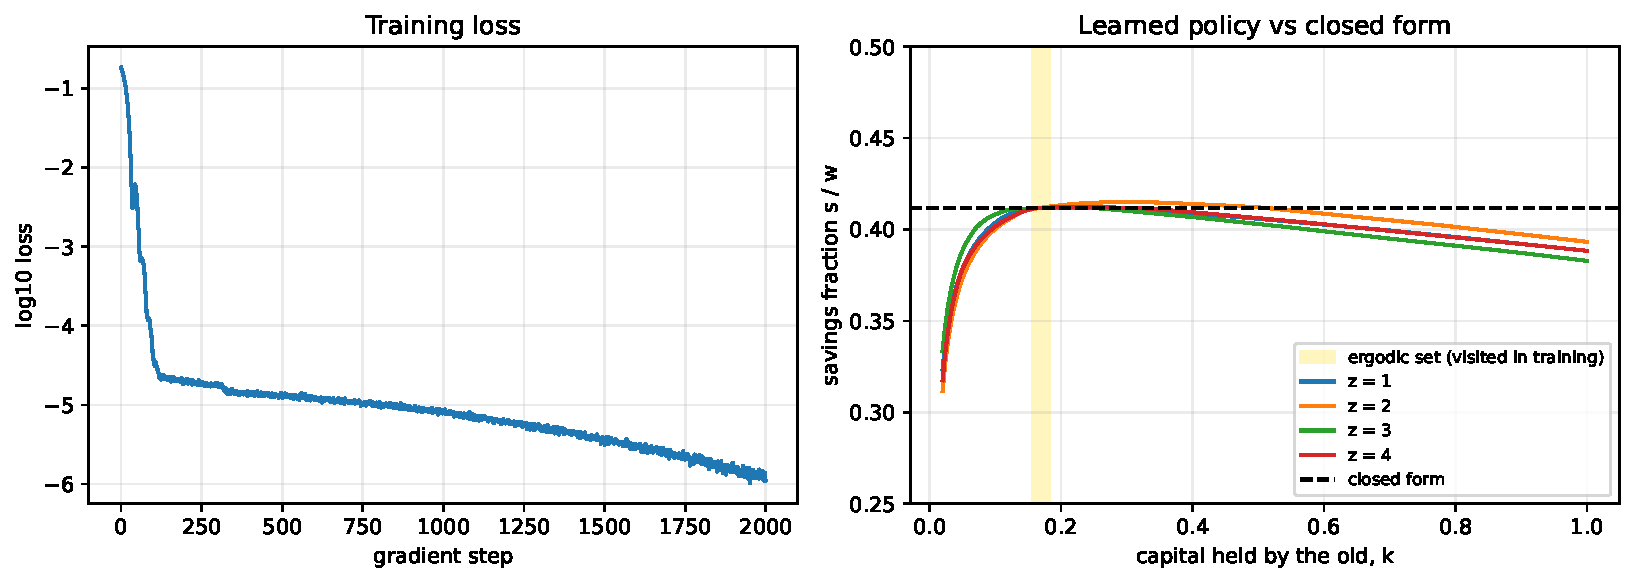
\includegraphics[height=2.35cm]{figures/olg2_savings_fraction.pdf}
\end{center}
\vspace{-0.5em}
{\scriptsize Left: training loss. Right: learned savings fraction against capital for each shock; closed form dashed, ergodic set shaded.}
\end{frame}


% =====================================================================
% Part II -- Analytic 6-agent model (Krueger & Kubler 2004)
% =====================================================================

\section{Part II: Analytic 6-agent OLG (Krueger \& K\"ubler, 2004)}

% --- II.1 Setup --------------------------------------------------------
\begin{frame}{II.1 Setup: the Analytic Model}
\footnotesize
\begin{columns}[T]
\column{0.58\textwidth}
\begin{itemize}\itemsep1pt
    \item Time discrete: $t = 0, 1, 2, \ldots, \infty$.
    \item Agents live for $A = \emphc{6}$ periods.
    \item \emphc{One representative household per cohort}; a new one is born every period.
    \item \emphc{No uncertainty about lifetime}: all agents live exactly $A$ periods.
    \item Exogenous aggregate shock $z_t \in \{1,2,3,4\}$ drawn \emphc{i.i.d.}\ with transition $\pi_{ss'} = 0.25$.
    \item \emphc{Log utility} $u(c) = \ln c$, chosen because it gives a \emphc{closed-form} equilibrium (Krueger \& K\"ubler, 2004).
    \item \emphc{Labor:} only the youngest cohort works: $\ell^1 = 1,\ \ell^h = 0$ for $h \ge 2$.
\end{itemize}

\column{0.41\textwidth}
\begin{block}{Shocks: $z_t = (\eta_t, \delta_t)$}
{\scriptsize\renewcommand{\arraystretch}{0.95}
\begin{tabular}{cccc}
\toprule
$z$ & $\eta(z)$ & $\delta(z)$ & $\pi$\\
\midrule
1 & 0.95 & 0.5 & 0.25\\
2 & 1.05 & 0.5 & 0.25\\
3 & 0.95 & 0.9 & 0.25\\
4 & 1.05 & 0.9 & 0.25\\
\bottomrule
\end{tabular}}
\end{block}

\begin{block}{Calibration}
{\scriptsize $\alpha = 0.3,\;\beta = 0.7,\;\gamma = 1$ (log); $\underline{a}=0$.}
\end{block}
\end{columns}
\end{frame}


% --- II.2 Households I -------------------------------------------------
\begin{frame}{II.2 Households: Preferences and the Savings Technology}
\small
Agents supply their labor \emphc{inelastically} for a market wage $w_t$.

\vspace{0.6em}
An agent \emphc{currently of age $h$} alive at $t$ maximises remaining time-separable discounted expected lifetime utility ($\beta < 1$):
\[
\mathbb{E}_t\!\left[\sum_{i=0}^{A-h} \beta^i \,\ln\!\bigl(c_{t+i}^{\,h+i}\bigr)\right] \qquad (1)
\]

\vspace{0.3em}
Households can save a unit of consumption to obtain a unit of capital good next period, denoted $a_t^{\,h}$.

\vspace{0.4em}
The savings become \emphc{capital in the next period}:
\[
a_t^{\,h} \;=\; k_{t+1}^{\,h+1}, \qquad \forall t,\ \forall h \in \{1, \ldots, A-1\}. \qquad (2)
\]
\end{frame}


% --- II.3 Households II ------------------------------------------------
\begin{frame}{II.3 Households: Constraints, Budget, Boundary}
\small
Households \emphc{cannot die with debt}.  Borrowing is bounded:
\[
a_t^{\,h} \;\ge\; \underline{a}. \qquad (3)
\]
In the analytic model we set $\underline{a} = 0$: \emphc{no borrowing} for any cohort.

\vspace{0.4em}
At time $t$, households sell their capital to the firm at market price $r_t > 0$.  The per-period \emphc{budget constraint} of cohort $h$ reads
\[
c_t^{\,h} \;+\; a_t^{\,h} \;=\; r_t\, k_t^{\,h} \;+\; \ell^h\, w_t. \qquad (4)
\]

\vspace{0.4em}
\emphc{Boundary conditions.}  Newborns enter with no inheritance, and the oldest cohort dies without saving anything:
\[
k_t^{\,1} \;=\; 0, \qquad\qquad a_t^{\,A} \;=\; 0.
\]
\end{frame}


% --- II.4 Firms & Markets ----------------------------------------------
\begin{frame}{II.4 Firms and Markets}
\small
There is a single representative firm with \emphc{Cobb--Douglas} production.

\vspace{0.3em}
TFP $\eta$ and depreciation $\delta$ depend on the exogenous shock $z$ alone (see II.1 table).

\vspace{0.3em}
Each period, \emphc{after the shock has realized}, the firm buys capital and hires labor to maximize profits, taking prices as given.

\vspace{0.4em}
The stochastic production function is
\[
f(K, L, z) \;=\; \eta(z)\, K^\alpha\, L^{1-\alpha} \;+\; K\bigl(1-\delta(z)\bigr).
\]

\vspace{0.4em}
There are \emphc{competitive spot markets} for the consumption good, capital, and labor.

\vspace{0.4em}
\textbf{Firm FOCs} (closed form, from Cobb--Douglas):
\[
w_t \;=\; (1-\alpha)\,\eta(z_t)\, K_t^{\alpha}\, L_t^{-\alpha}, \qquad
r_t \;=\; \alpha\,\eta(z_t)\, K_t^{\alpha-1}\, L_t^{1-\alpha} \;+\; \bigl(1-\delta(z_t)\bigr).
\]
{\footnotesize In the analytic model $L_t = \sum_{h=1}^A \ell^h = 1$ (only age-1 works), so the firm problem reduces to $\max_{K \ge 0} \eta(z) K^\alpha - (r_t - (1-\delta(z))) K$.  \emphc{Prices are a function of the state alone}, which is why the network never has to learn them here.}
\end{frame}


% --- II.5 Equilibrium definition ---------------------------------------
\begin{frame}{II.5 Competitive Equilibrium: Definition}
\footnotesize
\begin{block}{Definition 1 (competitive equilibrium)}
\vspace{-2pt}
Given initial conditions $z_0,\,\{k_0^{\,h}\}_{h=2}^{A}$, a competitive equilibrium is a collection of choices for households $\bigl\{(c_t^{\,h},\,a_t^{\,h})_{h=1}^{A}\bigr\}_{t=0}^{\infty}$, for the representative firm $(K_t, L_t)_{t=0}^{\infty}$, and prices $(r_t, w_t)_{t=0}^{\infty}$, such that:
\begin{enumerate}\itemsep1pt
    \item Given $(r_t, w_t)_{t\ge 0}$, household choices maximize the lifetime utility (1) subject to the savings-to-capital identity (2), the borrowing limit (3), and the per-period budget (4):\\[1pt]
    \mbox{}\hspace{1em}{\scriptsize $a_t^{\,h} = k_{t+1}^{\,h+1};\;\; a_t^{\,h} \ge \underline{a};\;\; c_t^{\,h} + a_t^{\,h} = r_t k_t^{\,h} + \ell^h w_t.$}
    \item Given $(r_t, w_t)$, the firm maximises profits:\\[1pt]
    \mbox{}\hspace{1em}$(K_t, L_t) \in \arg\max_{K, L \ge 0} f(K, L, z_t) - r_t K - w_t L$.
    \item \emphc{All markets clear:} for all $t$,\;\, $L_t = \sum_{h=1}^A \ell^h, \;\; K_t = \sum_{h=1}^A k_t^{\,h}.$
\end{enumerate}
\vspace{-2pt}
\end{block}
\end{frame}


% --- II.6 Equilibrium conditions: derivation first, result second ------
\begin{frame}{II.6 Household Optimality: Deriving the Euler Equation}
\footnotesize
Cohort $h$ at date $t$ chooses $\{c,a\}$ for its remaining $A-h+1$ periods.  Attach $\nu$ to the
budget constraint (4) and $\lambda\ge 0$ to the borrowing limit (3):
\[
\mathcal{L} = \mathbb{E}_t\sum_{i=0}^{A-h}\beta^i\Bigl[\ln c_{t+i}^{\,h+i}
 + \nu_{t+i}^{\,h+i}\bigl(r_{t+i}k_{t+i}^{\,h+i} + \ell^{h+i}w_{t+i} - c_{t+i}^{\,h+i} - a_{t+i}^{\,h+i}\bigr)
 + \lambda_{t+i}^{\,h+i}a_{t+i}^{\,h+i}\Bigr],
\quad k_{t+i+1}^{\,h+i+1} = a_{t+i}^{\,h+i}.
\]
\vspace{-6pt}
\begin{itemize}\itemsep1pt
    \item FOC in $c_t^{\,h}$: $\;\nu_t^{\,h} = 1/c_t^{\,h}$, the marginal utility of cash.
    \item FOC in $a_t^{\,h}$: $\;-\nu_t^{\,h} + \lambda_t^{\,h} + \beta\,\mathbb{E}_t\bigl[\nu_{t+1}^{\,h+1}\,r_{t+1}\bigr] = 0$,
          since $a_t^{\,h}$ becomes $k_{t+1}^{\,h+1}$ and earns $r_{t+1}$.
    \item Complementary slackness: $\lambda_t^{\,h}\ge 0$, $a_t^{\,h}\ge 0$, $\lambda_t^{\,h}a_t^{\,h}=0$.
\end{itemize}
\vspace{2pt}
\[
\boxed{\;\frac{1}{c_t^{\,h}} \;=\; \beta\,\mathbb{E}_t\!\left[\frac{r_{t+1}}{c_{t+1}^{\,h+1}}\right] + \lambda_t^{\,h}\;}
\qquad\text{terminal cohort: } a_t^{\,A}=0,\quad c_t^{\,A} = r_t k_t^{\,A}.
\]
\vspace{2pt}
{\scriptsize \emphc{Here $\lambda_t^{\,h}\equiv 0$}: no cohort has future labor income, only the newborn works
and only once, so there is nothing to borrow against and $a_t^{\,h}\ge 0$ never binds.  What remains is the
\emphc{interior} Euler equation.  Part III keeps $\lambda$ and adds a second multiplier.\par}
\end{frame}


% --- II.6a why a closed form ---------------------------------------------
\begin{frame}{II.6a Why This Model Has a Closed Form, and Why the Benchmark Does Not}
\footnotesize
\begin{columns}[T]
\column{0.55\textwidth}
\begin{block}{Two assumptions}
\vspace{-2pt}\begin{enumerate}\itemsep3pt
    \item \emphc{Log utility.}  $\mathbb{E}\ln(r'a) = \mathbb{E}\ln r' + \ln a$, so the savings rate does
          not depend on the return distribution: income and substitution effects of a return shock
          cancel. Persistent shocks would change nothing here; i.i.d.\ shocks only keep the aggregate
          dynamics simple.
    \item \emphc{No future labor income.}  Only the newborn works, once. Cash-on-hand
          $\text{inc}_t^{\,h} = r_t k_t^{\,h} + \ell^h w_t$ is the household's entire state, there is nothing
          to borrow against, and $\lambda\equiv 0$.
\end{enumerate}
\end{block}

\column{0.42\textwidth}
\begin{alertblock}{What the 56-cohort benchmark drops}
\vspace{-2pt}\begin{itemize}\itemsep2pt
    \item CRRA with $\gamma=2$: the return no longer separates, and a riskier $r'$ raises saving.
    \item Hump-shaped $\ell^h$: the young have wages ahead of them and want to borrow, so the
          constraint binds, and so does a collateral constraint on bonds.
\end{itemize}
\vspace{2pt}
No closed form; multipliers in the network; a numerical solver is needed.
\end{alertblock}
\end{columns}
\end{frame}


% --- II.6b backward induction --------------------------------------------
\begin{frame}{II.6b Backward Induction to $\beta_h$}
\small
Write $\text{inc}$ for cash-on-hand and $V_h(\text{inc})$ for the value of a cohort of age $h$.
\begin{itemize}\itemsep4pt
    \item \textbf{Age $A$:} no tomorrow. $c = \text{inc}$, \; $V_A(\text{inc}) = \ln \text{inc}$.
    \item \textbf{Age $A-1$:} $\max_a\;\ln(\text{inc}-a) + \beta\,\mathbb{E}\ln(r'a)$. FOC $\tfrac{1}{\text{inc}-a}=\tfrac{\beta}{a}$
          $\Rightarrow a = \tfrac{\beta}{1+\beta}\text{inc}$, \; $V_{A-1}(\text{inc}) = (1+\beta)\ln \text{inc} + \text{const}$.
    \item \textbf{Age $A-2$:} $\max_a\;\ln(\text{inc}-a) + \beta(1+\beta)\,\mathbb{E}\ln(r'a)$
          $\Rightarrow a = \tfrac{\beta+\beta^2}{1+\beta+\beta^2}\text{inc}$, \; $V_{A-2}(\text{inc}) = (1+\beta+\beta^2)\ln \text{inc} + \text{const}$.
    \item \textbf{Age $h$,} by induction:
\end{itemize}
\[
\boxed{\;\beta_h \;=\; \frac{a}{\text{inc}} \;=\; \frac{\beta+\beta^2+\cdots+\beta^{A-h}}{1+\beta+\cdots+\beta^{A-h}}
\;=\; \beta\,\frac{1-\beta^{A-h}}{1-\beta^{A-h+1}},\qquad h=1,\ldots,A-1.\;}
\]
\vspace{0.2em}
{\footnotesize The constant absorbs $\mathbb{E}\ln r'$ at every step, which is why the return distribution never reaches the decision. The policy is a fixed fraction of $\text{inc}_t^{\,h}$, which is why the sigmoid savings-fraction head of II.9 has the same shape as the closed form.}
\end{frame}


% --- II.7 Cost function ------------------------------------------------
\begin{frame}{II.7 The DEQN Cost Function}
\footnotesize
\begin{block}{Explicit cost function}
\[
\boxed{\;\Loss_{D_{\text{train}}}(\theta) \;:=\; \frac{1}{|D_{\text{train}}|}\;\frac{1}{A-1}\,
\sum_{x_j \in D_{\text{train}}}\;\sum_{i=1}^{A-1} \bigl(e_{\text{REE}}^{\,i}(x_j)\bigr)^2\;}
\]
\end{block}

\vspace{0.3em}
\textbf{Relative Euler-equation residual} (cohort $i$):
\[
e_{\text{REE}}^{\,i}(x_j) \;:=\;
\frac{\Bigl(u'\Bigr)^{-1}\!\!\left(\beta\,\E{r\bigl(\hat x_{j,+}\bigr)\,u'\bigl(\hat c^{\,i+1}(\hat x_{j,+})\bigr)}\right)}{\hat c^{\,i}(x_j)} \;-\; 1.
\]

\textbf{Next state and expectation.}  $\hat x_{j,+} = \bigl(z_+,\; 0,\; \hat a^{\,[1:A-1]}(x_j)\bigr)$, the newborn entering with $k^1 = 0$; $\mathbb{E}$ is the exact four-term sum over $z_+$.

\textbf{No market-clearing residual.}  Next period's capital is defined as $K_{t+1}=\sum_h \hat a^{\,h}(x_j)$, so the capital market clears by construction. Part III needs one for bonds.

\vspace{0.2em}
{\scriptsize \emphc{In the code} (\texttt{04\_01}) the loss carries two feasibility penalties, on negative consumption and negative aggregate capital, weight $10$; they keep early training out of the region where $\ln c$ is undefined and are inactive thereafter.}

\end{frame}


% --- II.7a where the network appears twice ------------------------------
\begin{frame}{II.7a Where the Network Appears \emphc{Twice}}
\footnotesize
\centering
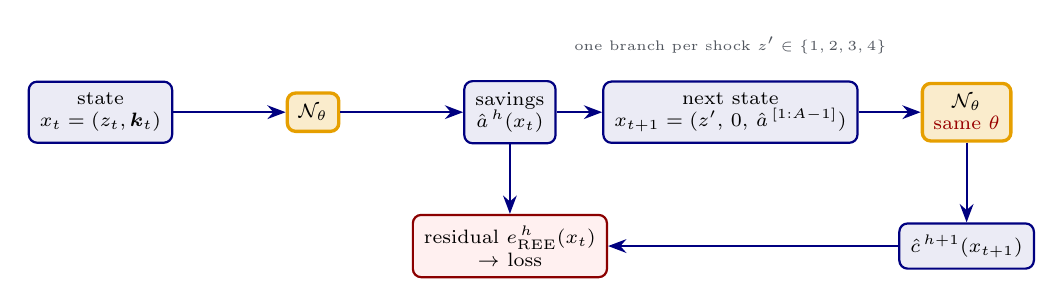
\begin{tikzpicture}[
    node distance=6mm, >=Stealth,
    st/.style={rectangle, draw=uzhblue, thick, rounded corners=3pt, fill=uzhblue!8,
               align=center, font=\scriptsize, inner sep=4pt},
    nn/.style={rectangle, draw=softorange, very thick, rounded corners=3pt, fill=softorange!20,
               align=center, font=\scriptsize, inner sep=4pt},
    rs/.style={rectangle, draw=darkred, thick, rounded corners=3pt, fill=red!6,
               align=center, font=\scriptsize, inner sep=4pt},
    arr/.style={->, thick, uzhblue}
]
\node[st] (x)  at (0,0)    {state\\$x_t=(z_t,\bm{k}_t)$};
\node[nn] (n1) at (2.7,0)  {$\N_\theta$};
\node[st] (a)  at (5.2,0)  {savings\\$\hat a^{\,h}(x_t)$};
\node[st] (xp) at (8.0,0)  {next state\\$x_{t+1}=(z',\,0,\,\hat a^{\,[1:A-1]})$};
\node[nn] (n2) at (11.0,0) {$\N_\theta$\\\emphc{same $\theta$}};
\node[st] (cp) at (11.0,-1.7) {$\hat c^{\,h+1}(x_{t+1})$};
\node[rs] (e)  at (5.2,-1.7) {residual $e^{\,h}_{\text{REE}}(x_t)$\\$\to$ loss};
\node[font=\tiny, uzhgreydark] at (8.0,0.85) {one branch per shock $z'\in\{1,2,3,4\}$};

\draw[arr] (x) -- (n1);  \draw[arr] (n1) -- (a);  \draw[arr] (a) -- (xp);
\draw[arr] (xp) -- (n2); \draw[arr] (n2) -- (cp); \draw[arr] (cp) -- (e);
\draw[arr] (a) -- (e);
\end{tikzpicture}

\vspace{0.2em}
\raggedright
Cohort $h$'s Euler equation needs $c_{t+1}^{\,h+1}$, the consumption of a household \emph{one year older}
next period.  It is not observed; the network supplies it: one call at $x_t$, one call at each
successor state.  \emphc{Five forward passes per residual}, all with the same $\theta$.

\vspace{0.3em}
\begin{alertblock}{The loss is a fixed point, not a regression}
\vspace{-2pt}
The loss is a \emphc{fixed-point condition on $\theta$}, not a regression: there is no target to fit,
only the requirement that the network be consistent with itself one period ahead.  Gradients flow
through \emph{both} calls.  This is also why there is no contraction theorem and the stopping rule
has to be empirical (Session 2, Algorithm 1).
\end{alertblock}
\end{frame}


% --- II.8 From a sequence to a function, and the FREE it defines --------
\begin{frame}{II.8 From a Sequence to a Function (FREE)}
\scriptsize
Definition 1 describes an equilibrium as \emph{sequences} $\{c_t^{\,h}, a_t^{\,h}, r_t, w_t\}_{t\ge 0}$.
A network represents a \emph{function}.  The link is a sufficient state.

\vspace{-2pt}
\begin{block}{$(z_t,\bm{k}_t)$ is all a household needs to know}
\vspace{-3pt}\begin{itemize}\itemsep0pt
    \item \emph{Today:} $K_t=\sum_h k_t^{\,h}$ and $z_t$ pin down $(r_t,w_t)$, hence every cohort's cash-on-hand.
    \item \emph{Tomorrow:} if behaviour is the same in the same state, $(z_{t+1},\bm{k}_{t+1})$ depends only on
          $(z_t,\bm{k}_t)$, the shock, and that behaviour.
\end{itemize}
\vspace{-3pt}
\end{block}
\vspace{-3pt}
So we look for a \emphc{recursive} equilibrium: time-invariant policies with $\bm{k}' = (0,\,a^1(z,\bm{k}),\ldots,a^{A-1}(z,\bm{k}))$.

\vspace{-1pt}
\begin{exampleblock}{Functional rational expectations equilibrium (FREE)}
\vspace{-6pt}
\[
f:\;\{1,2,3,4\}\times \R^{A} \to \R^{\,A-1},
\quad
f(z_t, \bm{k}_t) = \bigl[\,a_t^{\,1},\ldots,a_t^{\,A-1}\,\bigr]^{\!\top},
\quad
\beta\,\E{\frac{r_{t+1}\,u'(c_{t+1}^{\,h+1})}{u'(c_t^{\,h})}} - 1 = 0 \;\;\forall h,
\]
\vspace{-9pt}
\begin{center}i.e.\ $G\bigl([z_t,\bm{k}_t],\,f([z_t,\bm{k}_t])\bigr)=\bm{0}$ at \emph{every} state.\end{center}
\vspace{-6pt}\end{exampleblock}
\vspace{-3pt}
{\scriptsize Existence and stationarity are \emph{assumed}; in Part II the closed form is such a function, so here the assumption is verified.\quad \emphc{$f$ is the unknown the equilibrium defines; $\N_\theta$ on the next slide is the parametric family we search in.}}
\end{frame}


% --- II.9 Architecture --------------------------------------------------
\begin{frame}{II.9 Deep Equilibrium Net: Architecture (Analytic)}
\small
\begin{columns}[T,totalwidth=0.96\textwidth]
\column{0.46\textwidth}
\[
\N_\theta:\;\{1,2,3,4\}\times\R^A \to \R^{A-1}
\]
\[
\N_\theta\!\left(\!\begin{bmatrix} z_t \\ \bm{k}_t\end{bmatrix}\!\right) \;=\;
\left[
\begin{array}{l}
a_t^{\,1}\\ a_t^{\,2}\\ \vdots\\ a_t^{\,A-1}
\end{array}
\right]
\]
such that
\[
G\!\left(\!\begin{bmatrix} z_t \\ \bm{k}_t\end{bmatrix},\; \N_\theta\!\left(\!\begin{bmatrix} z_t \\ \bm{k}_t\end{bmatrix}\!\right)\right) \;\approx\; \bm{0}.
\]
{\footnotesize \emphc{Sigmoid savings-fraction} output $\Rightarrow$ $0 \le a_t^{\,h} \le \mathrm{inc}_t^{\,h}$ \emphc{by construction}, so $a_t^{\,h}\ge 0$ (borrowing constraint) and $c_t^{\,h}\ge 0$ both hold at every iteration without an explicit multiplier.}

\column{0.48\textwidth}
\centering
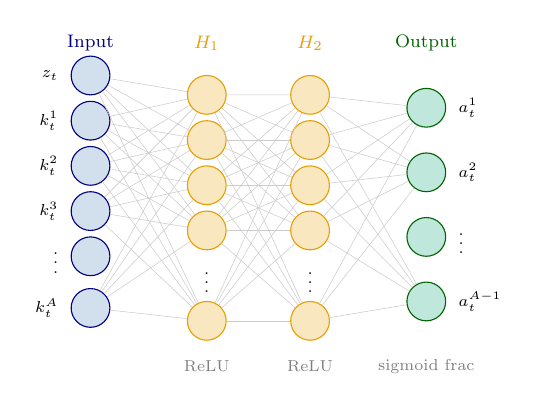
\begin{tikzpicture}[scale=0.82, every node/.style={transform shape},
    inn/.style={circle, draw=uzhblue, fill=softblue!25, minimum size=6mm, inner sep=0pt, font=\scriptsize},
    hd/.style={circle, draw=softorange, fill=softorange!25, minimum size=6mm, inner sep=0pt, font=\scriptsize},
    outt/.style={circle, draw=darkgreen, fill=softgreen!25, minimum size=6mm, inner sep=0pt, font=\scriptsize},
    dots/.style={font=\scriptsize},
    >=Stealth
]
\node[font=\footnotesize, uzhblue]     at (0, 3.4) {Input};
\node[font=\footnotesize, softorange]  at (1.8, 3.4) {$H_1$};
\node[font=\footnotesize, softorange]  at (3.4, 3.4) {$H_2$};
\node[font=\footnotesize, darkgreen]   at (5.2, 3.4) {Output};

\foreach \i/\y/\lab in {a/2.9/$z_t$, b/2.2/$k^1_t$, c/1.5/$k^2_t$, d/0.8/$k^3_t$, e/0.1/$\vdots$, f/-0.7/$k^A_t$} {
    \node[inn] (In\i) at (0, \y) {};
    \node[left=2pt of In\i, font=\scriptsize] {\lab};
}

\foreach \i/\y in {a/2.6, b/1.9, c/1.2, d/0.5, e/-0.9} {
    \node[hd] (HOne\i) at (1.8, \y) {};
    \node[hd] (HTwo\i) at (3.4, \y) {};
}
\node[dots] at (1.8, -0.2) {$\vdots$};
\node[dots] at (3.4, -0.2) {$\vdots$};

\foreach \i/\y/\lab in {a/2.4/$a_t^1$, b/1.4/$a_t^2$, c/0.4/$\vdots$, d/-0.6/$a_t^{A-1}$} {
    \node[outt] (Out\i) at (5.2, \y) {};
    \node[right=2pt of Out\i, font=\scriptsize] {\lab};
}

% connections input -> H1
\foreach \a in {a, b, c, d, f}
    \foreach \b in {a, b, c, d, e}
        \draw[gray!40, very thin] (In\a) -- (HOne\b);
% H1 -> H2
\foreach \a in {a, b, c, d, e}
    \foreach \b in {a, b, c, d, e}
        \draw[gray!40, very thin] (HOne\a) -- (HTwo\b);
% H2 -> output
\foreach \a in {a, b, c, d, e}
    \foreach \b in {a, b, d}
        \draw[gray!40, very thin] (HTwo\a) -- (Out\b);

\node[font=\scriptsize, gray] at (1.8, -1.6) {ReLU};
\node[font=\scriptsize, gray] at (3.4, -1.6) {ReLU};
\node[font=\scriptsize, gray] at (5.2, -1.6) {sigmoid frac};
\end{tikzpicture}

{\footnotesize 2 hidden layers $\times$ (100, 50) units; single forward pass.}
\end{columns}
\end{frame}


% --- Hand-over to the analytic-model notebook -------------------------
\begin{frame}{Companion Notebook Hand-over}
\scriptsize
\emphc{Open notebook \texttt{04\_01\_OLG\_Analytic\_DEQN\_persistent.ipynb}} (the persistent-simulation primary; the exogenous-sampling companion is \texttt{04\_04\_OLG\_Analytic\_DEQN\_exogenous.ipynb}; if you skipped it, \texttt{04\_00} is the two-period warm-up with the same structure in sixty lines).  It implements the model, equilibrium conditions, loss, FREE map, architecture, training, and validation covered in Part II.
\vspace{-2pt}
\begin{block}{Cell-to-slide map}
\vspace{-4pt}
\begin{center}\renewcommand{\arraystretch}{0.85}
{\scriptsize
\begin{tabular}{ll}
\toprule
\textbf{Deck slide} & \textbf{Notebook section} \\
\midrule
II.1--II.6 Model and equilibrium        & \S 1--4 \;parameters, closed form, state, network \\
II.7--II.9 Loss, FREE, architecture     & \S 5--6 \;\texttt{compute\_residuals()}, training states \\
II.10--II.12 Training/validation        & \S 7--10 \;training loop, diagnostics, policy stability, closed-form checks \\
\bottomrule
\end{tabular}}
\end{center}
\vspace{-4pt}
\end{block}
\end{frame}


% --- II.10 Sampling + training loop -----------------------------------
\begin{frame}{II.10 Sampling and the Training Loop}
\small
\begin{block}{The DEQN training algorithm (Azinovic, Gaegauf \& Scheidegger, 2022), applied to OLG}
\vspace{-2pt}
\begin{enumerate}\itemsep2pt
    \item \emphc{Initialisation.}  Sample a set of initial states $D_0 = \{x_j^{\,0}\}_{j=1}^{N}$; initialise $\theta^0$.
    \item \emphc{Episode $k$.}
    \begin{enumerate}
        \item[(a)] \textbf{Simulate.}  Draw fresh shocks $\{z_{+,j}\}$ from $\pi$; roll the states forward one period using the \emphc{current} policy $\N_{\theta^k}$:
        $x_j^{\,k+1} = \bigl(z_{+,j},\,0,\,\N_{\theta^k}^{[1:A-1]}(x_j^{\,k})\bigr)$.
        \item[(b)] \textbf{Mini-batch SGD.}  Take $\texttt{steps}$ Adam steps on $\Loss_{D_k}(\theta)$ using mini-batches from $D_k$.
    \end{enumerate}
    \item After a fixed number of episodes, check that the policy has stopped moving on held-out states.
\end{enumerate}
\end{block}

\vspace{0.2em}
\textbf{Definitions.}  \emphc{Episode} = one simulate-then-train pass.  \emphc{Epoch} = one pass through the full training set.

\vspace{0.2em}
{\footnotesize Algorithm 1 of Session 2, unchanged: only the state $x$ and the residual $G$ are OLG-specific.  Sampling from the ergodic set of the current policy concentrates the cost function on states the economy visits.}
\end{frame}


% --- II.11 Training results -------------------------------------------
\begin{frame}{II.11 Training Results: Analytic Model (teaching-mode run)}
\footnotesize
\centering
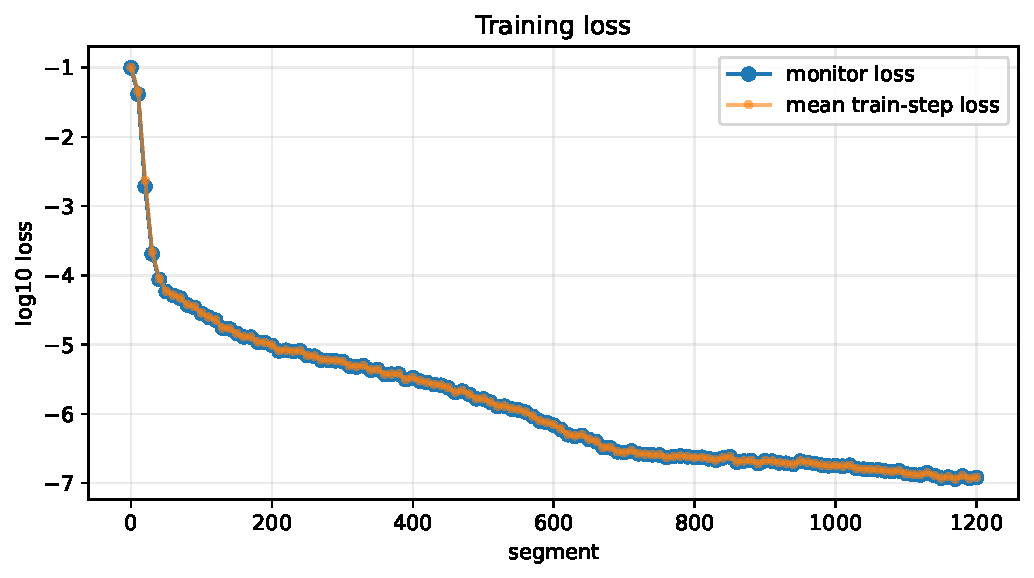
\includegraphics[height=3.0cm]{figures/olg6_loss.pdf}\hfill
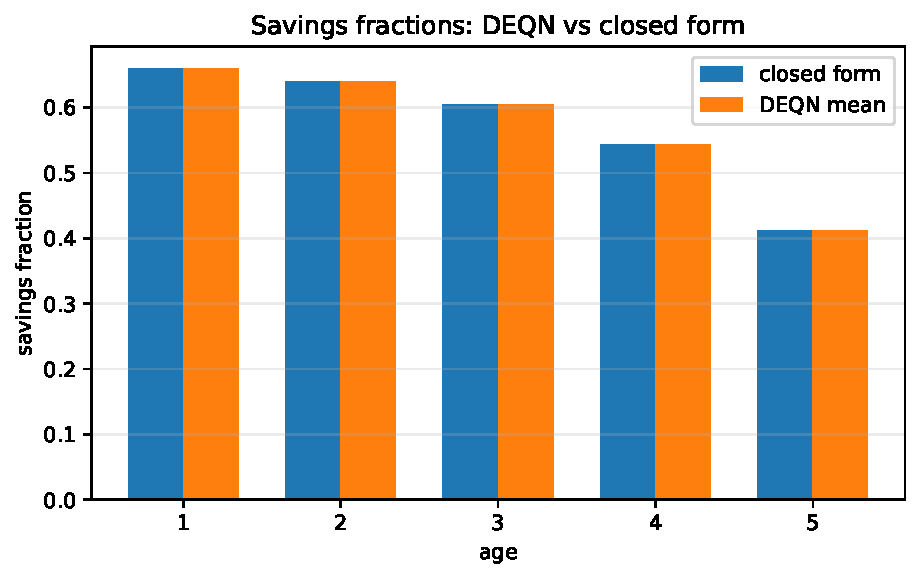
\includegraphics[height=3.0cm]{figures/olg6_savings_bars.pdf}

\vspace{-0.1em}
\begin{block}{Reading the plots}
\vspace{-2pt}
{\scriptsize\emphc{Left:} monitor loss and mean train-step loss per segment, $\log_{10}$ scale; the training states are re-simulated each segment.\\
\emphc{Right:} mean savings fraction by cohort against the closed form $\beta_h$, matched to $1.0\times 10^{-5}$.}
\vspace{-2pt}
\end{block}
\vspace{-5pt}
{\scriptsize \texttt{04\_01} at \texttt{RUN\_MODE = "teaching"}, eleven minutes on a laptop CPU; mean relative Euler error $2.5\times10^{-4}$ on out-of-sample simulated states.  Use \texttt{"smoke"} ($\sim$2.5 min) in class.}
\end{frame}


% --- II.12 Finger exercise --------------------------------------------
\begin{frame}{\emphc{Finger Exercise:} Closed-Form Savings Rates}
\small
\textbf{Task (3 minutes).}  Take $\beta_h$ as derived on II.6b,
\[
\beta_h \;=\; \frac{a_t^h}{\text{inc}_t^h} \;=\; \beta\,\frac{1 - \beta^{A-h}}{1 - \beta^{A-h+1}},
\qquad \text{inc}_t^h = r_t k_t^h + \ell^h w_t, \qquad h = 1, \ldots, A-1,
\]
and evaluate it at $\beta = 0.7$, $A = 6$: compute $\beta_1, \beta_2, \ldots, \beta_5$.

\vspace{0.6em}
\textbf{Then interpret.}
\begin{itemize}\itemsep4pt
\item What happens to the savings \emph{rate} as a cohort approaches retirement, and why?
\item Why do younger cohorts save more as a rate, even though they are poorer?
\item These five numbers are the \emphc{validation target} of Krueger \& K\"ubler (2004): the DEQN
      has to reproduce them without ever being told what they are.
\end{itemize}
\end{frame}


\begin{frame}{\emphc{Solution:} Closed-Form Savings Rates}
\footnotesize
\[
\beta_h \;=\; 0.7 \cdot \frac{1 - 0.7^{\,6-h}}{1 - 0.7^{\,7-h}}
\]

\vspace{-0.1em}
\begin{center}\renewcommand{\arraystretch}{0.95}
\begin{tabular}{ccc}
\toprule
Cohort $h$ & Periods remaining ($A-h$) & Savings rate $\beta_h$\\
\midrule
1 & 5 & $0.7\cdot(1-0.7^5)/(1-0.7^6) \approx 0.660$ \\
2 & 4 & $0.7\cdot(1-0.7^4)/(1-0.7^5) \approx 0.639$ \\
3 & 3 & $0.7\cdot(1-0.7^3)/(1-0.7^4) \approx 0.605$ \\
4 & 2 & $0.7\cdot(1-0.7^2)/(1-0.7^3) \approx 0.543$ \\
5 & 1 & $0.7\cdot(1-0.7)/(1-0.7^2) \approx 0.412$ \\
6 & 0 & $0$ (consumes everything)\\
\bottomrule
\end{tabular}\end{center}

\vspace{-0.1em}
\begin{block}{Interpretation}
\vspace{-3pt}\begin{itemize}\itemsep0pt
    \item Savings rate \emphc{monotonically declines} with age: as the horizon shrinks, saving less is optimal.
    \item Youngest cohort saves \emphc{$\sim 66\%$} of its income, longest horizon to enjoy the returns.
    \item At $A$: terminal boundary $a^A = 0$, consume everything.
\end{itemize}
\end{block}
\end{frame}


% --- II.12 Validation --------------------------------------------------
\begin{frame}{II.12 DEQN vs.\ Analytical Solution}
\footnotesize
\centering
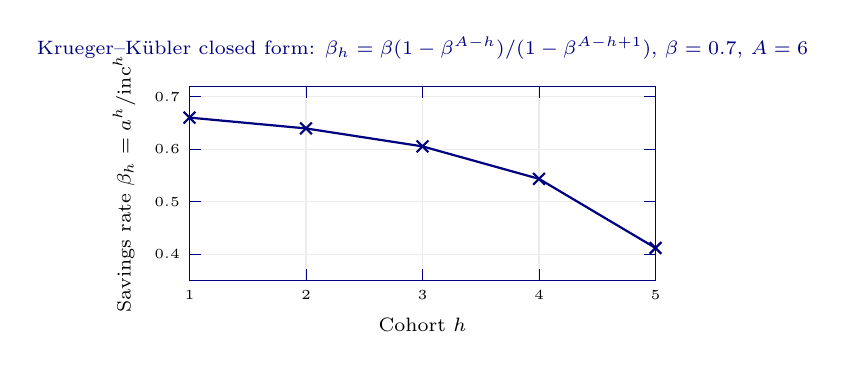
\begin{tikzpicture}
\begin{axis}[
    width=7.5cm, height=4.05cm,
    xlabel={Cohort $h$}, ylabel={Savings rate $\beta_h = a^h / \text{inc}^h$},
    xmin=1, xmax=5, ymin=0.35, ymax=0.72,
    xtick={1,2,3,4,5},
    grid=major, grid style={gray!15},
    axis line style={uzhblue}, tick style={uzhblue},
    label style={font=\scriptsize}, ticklabel style={font=\tiny},
    title style={font=\scriptsize, uzhblue},
    title={Krueger--K\"ubler closed form: $\beta_h = \beta(1-\beta^{A-h})/(1-\beta^{A-h+1})$, $\beta=0.7,\,A=6$}
]
\addplot[uzhblue, thick, mark=x, mark size=3pt] coordinates {
    (1,0.6600) (2,0.6394) (3,0.6052) (4,0.5434) (5,0.4118)
};
\end{axis}
\end{tikzpicture}

\vspace{0.2em}
\begin{block}{Validation strategy}
\vspace{-2pt}
The points are the exact closed form. The DEQN should reproduce them cohort by cohort; the next slide checks it state by state. Production target in AGS (2022): mean relative Euler error below $10^{-3}$.
\end{block}
\end{frame}

\begin{frame}{II.12$'$ Policy Functions State by State}
\centering
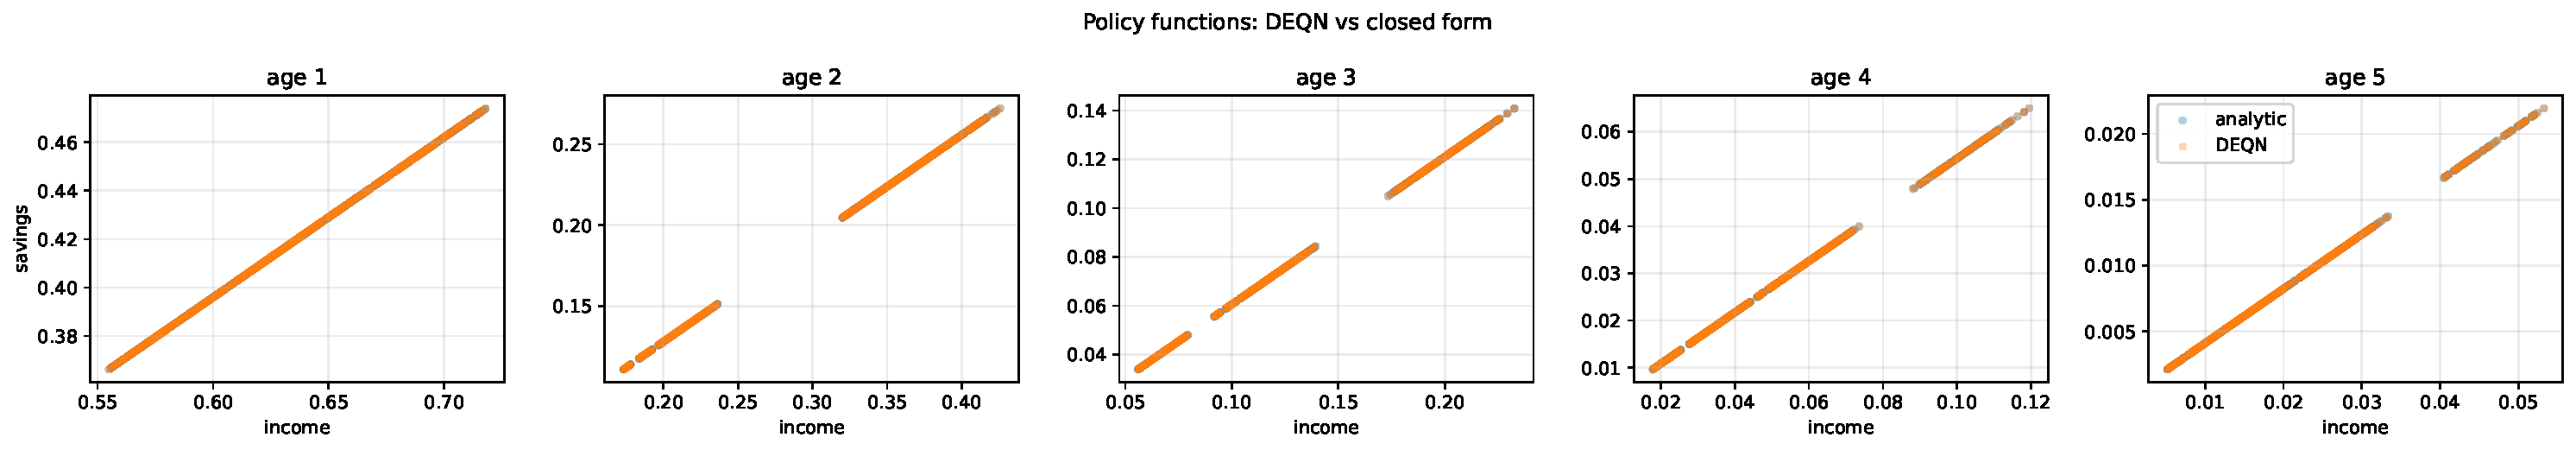
\includegraphics[width=0.98\textwidth]{figures/olg6_policy_scatter.pdf}

\vspace{0.3em}
{\small One panel per cohort: savings $a^h$ against cash-on-hand $\text{inc}^h$ on the simulated ergodic set. The closed form is a line through the origin with slope $\beta_h$; the DEQN should lie on it at every income level.}

\vspace{0.2em}
{\footnotesize The ergodic gross return is about $0.69$, below one because $\delta\in\{0.5,0.9\}$, and the young still save two thirds of their wage: capital is the only store of value in this economy.}
\end{frame}


\begin{frame}{II. Take-away and Hands-on}
\footnotesize
\begin{block}{What we just did}
\begin{enumerate}\itemsep1pt
    \item OLG model with 6 cohorts, log utility, 4 i.i.d.\ shocks (II.1--II.4).
    \item Equilibrium definition + conditions (II.5--II.6).
    \item Conditions $\to$ \emphc{cost function} (II.7).
    \item Equilibrium map $f$ $\to$ neural network $\N_\theta$ (II.8--II.9).
    \item Trained by sampling + SGD (II.10--II.11), \emphc{validated} against the closed form (II.12).
\end{enumerate}
\end{block}

\begin{block}{Hands-on}
Open \texttt{04\_01\_OLG\_Analytic\_DEQN\_persistent.ipynb}.  Run \texttt{RUN\_MODE = "smoke"} ($\sim$2.5 min) now; the stored outputs are already the converged \texttt{"teaching"} run ($\sim$11 min on a laptop CPU), and \texttt{"production"} targets the accuracy of AGS (2022), Table~3.  Both notebooks expose a \texttt{SAMPLING\_MODE = "simulation" / "exogenous"} switch (the persistent primary uses \texttt{"simulation"}, the companion \texttt{04\_04\_OLG\_Analytic\_DEQN\_exogenous.ipynb} uses \texttt{"exogenous"}); the model and loss are identical, only the training states differ.
\end{block}
\end{frame}


% =====================================================================
% Part III -- Benchmark (AGS 2022 leading example), slides only
% =====================================================================

\section{Part III: Benchmark 56-cohort OLG (AGS 2022 \S 3)}

% --- III.1 What changes at research scale ------------------------------
\begin{frame}{III.1 What Changes at Research Scale: AGS (2022), \S 3}
\scriptsize
\begin{columns}[T]
\column{0.56\textwidth}
\emphc{Same recipe as Part II.  Seven things change:}
\begin{itemize}\itemsep0pt
    \item $A = \emphc{56}$ periods (ages 25--80), one period $=$ one year.
    \item CRRA $u(c)=c^{1-\gamma}/(1-\gamma)$, $\gamma = 2$, \emphc{not} log.
    \item \emphc{Hump-shaped} labor $\ell^h$ (right), so the young have wages ahead of them.
    \item \emphc{Persistent} Markov shocks on $(\eta,\delta)$, not i.i.d.
    \item \emphc{Two assets}: capital $k^h$ and a one-period bond $b^h$ in zero net supply,
          $\sum_h b_t^h = 0$, traded at an endogenous price $p_t$.
    \item \emphc{Two constraints}: $k'^h \ge 0$ and $k'^h + \kappa b'^h \ge 0$.
    \item Capital adjustment costs $\Psi^h = \tfrac{\zeta}{2}(k'^h - r k^h)^2$.
\end{itemize}
\vspace{2pt}
{\scriptsize Budget: $c_t^{h} + k_{t+1}^{h+1} + p_t b_{t+1}^{h+1} + \Psi_t^h = r_t k_t^{h} + b_t^{h} + \ell^{h} w_t$.
Born and die with nothing.  Three markets clear: labor, capital, \emphc{and bonds}.}

\column{0.42\textwidth}
\centering
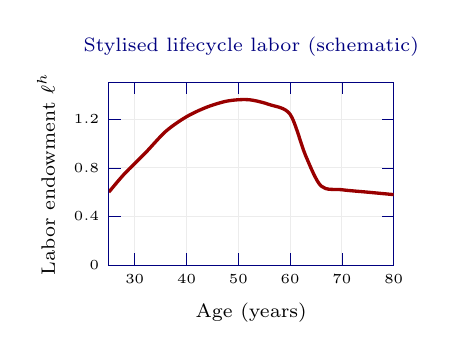
\begin{tikzpicture}
\begin{axis}[
    width=5.2cm, height=3.9cm,
    xlabel={Age (years)}, ylabel={Labor endowment $\ell^h$},
    xmin=25, xmax=80, ymin=0, ymax=1.5,
    xtick={30,40,50,60,70,80}, ytick={0, 0.4, 0.8, 1.2},
    grid=major, grid style={gray!15},
    axis line style={uzhblue}, tick style={uzhblue},
    label style={font=\scriptsize}, ticklabel style={font=\tiny},
    title style={font=\scriptsize, uzhblue},
    title={Stylised lifecycle labor (schematic)}
]
\addplot[harvardcrimson, very thick, smooth] coordinates {
    (25,0.60) (28,0.75) (32,0.92) (36,1.10) (40,1.22)
    (44,1.30) (48,1.35) (52,1.36) (56,1.32) (60,1.24)
    (63,0.90) (66,0.65) (70,0.62) (75,0.60) (80,0.58)
};
\end{axis}
\end{tikzpicture}

{\scriptsize \emphc{Both assumptions of II.6a fail here.}  CRRA removes the separation of return and choice;
future wages give the young a reason to borrow, so the constraints bind and multipliers are back.}
\end{columns}
\end{frame}


% --- III.2 Equilibrium conditions and the multipliers --------------------
\begin{frame}{III.2 Equilibrium Conditions, and Where Each Multiplier Lands}
\scriptsize
Same Lagrangian as II.6, with $\lambda_b\ge 0$ on $k'\ge 0$ and $\mu\ge 0$ on $k'+\kappa b'\ge 0$.
Write $\mathcal{A}_t^h := 1 + \zeta\,(k'^h_t - r_t k_t^h)$ for the marginal adjustment-cost wedge.
\vspace{-2pt}
\[
\frac{\partial}{\partial k'}:\;\;
u'(c_t^h)\,\mathcal{A}_t^h = \beta\,\E{u'(c_{t+1}^{h+1})\,r_{t+1}\,\mathcal{A}_{t+1}^{h+1}}
+ \ubr{1\cdot\lambda_b^h}{$\partial k'/\partial k'$} + \ubr{1\cdot\mu^h}{$\partial(k'+\kappa b')/\partial k'$}
\]
\vspace{-10pt}
\[
\frac{\partial}{\partial b'}:\;\;
u'(c_t^h)\,p_t = \beta\,\E{u'(c_{t+1}^{h+1})} + \ubr{\kappa\,\mu^h}{$\partial(k'+\kappa b')/\partial b'$}
\qquad (\lambda_b \text{ absent: } b' \text{ is not in that constraint})
\]
\vspace{-4pt}
\begin{block}{The general rule}
\vspace{-2pt}
A multiplier enters each first-order condition weighted by \emphc{its constraint's derivative in that
instrument}.  The collateral constraint contains both assets, so $\mu$ appears twice, scaled by $\kappa$
in the bond equation; the borrowing constraint contains only capital, so $\lambda_b$ appears once.
\vspace{-2pt}
\end{block}
\vspace{-3pt}
\textbf{Two KKT triples per cohort:}\;
$\lambda_b^h \ge 0,\; k'^h \ge 0,\; \lambda_b^h k'^h = 0$; \quad
$\mu^h \ge 0,\; k'^h{+}\kappa b'^h \ge 0,\; \mu^h(k'^h{+}\kappa b'^h) = 0$.

\vspace{-1pt}
{\scriptsize With $\mu = 0$ the bond equation is $p = \beta\,\mathbb{E}[u'(c')]/u'(c)$, the price of a riskless
claim; a binding collateral constraint adds the shadow value $\kappa\mu/u'(c)$ that a constrained cohort
will pay on top.}
\end{frame}


% --- III.3 The cost function and the network at scale --------------------
\begin{frame}{III.3 The Same Loss, at Twenty Times the Size}
\footnotesize
\begin{block}{Stack everything, exactly as in II.7}
\vspace{-6pt}
\[
\Loss(\theta) = \operatorname{mean}_{x_j \in D}\Biggl[\;\sum_{h=1}^{A-1}
\underbrace{\bigl(e_{\text{REE},k}^{h}\bigr)^2 + \bigl(e_{\text{REE},b}^{h}\bigr)^2
+ \underbrace{\bigl(\lambda_b^h k'^h\bigr)^2 + \bigl(\mu^h q^h\bigr)^2}_{\text{KKT, product form}}}_{\text{per cohort}}
\;+\; \Bigl(\underbrace{\textstyle\sum_h \hat b'^h}_{\text{bond market}}\Bigr)^2\Biggr]
\]
\vspace{-8pt}
\end{block}
\vspace{-4pt}
\begin{columns}[T]
\column{0.52\textwidth}
\textbf{The network.}
\[
\N_\theta:\;\R^{240} \longrightarrow \R^{221}
\]
\vspace{-10pt}
\begin{itemize}\itemsep0pt
    \item minimal state $113$; input $12+4A = 236$ after engineered aggregates and transition probabilities (AGS 2022, \S 4.3)
    \item output $4\times 55 + 1 = \emphc{221}$: $\hat k'^h$, $\hat\lambda_b^h$, $\hat b'^h$, $\hat\mu^h$, and the
          \emphc{bond price $\hat p_t$}, an equilibrium price the network must learn
    \item two ReLU layers of $1000$ units
\end{itemize}
\column{0.46\textwidth}
\begin{alertblock}{Nothing conceptually new}
\vspace{-2pt}
Part II had $A-1 = 5$ residuals per state.  This has $221$.  The recipe, the cost function, the
simulate-and-train loop, and the diagnostics are \emph{identical}.  What changes is how hard the
optimisation is.
\vspace{-2pt}
\end{alertblock}
\end{columns}
\end{frame}


% =====================================================================
% Part IV -- Wrap-up
% =====================================================================

\section{Part IV: Wrap-up}

\begin{frame}{Summary}
\scriptsize
\begin{block}{What we accomplished}
\vspace{-2pt}\begin{enumerate}\itemsep0pt
    \item OLG models: a finite-dimensional family of heterogeneous-agent models, suited to DEQNs.
    \item Applied the DEQN recipe \emphc{three times}:
    \begin{itemize}\itemsep0pt
        \item \emphc{Part I\textonehalf:} Diamond's two-period model, one Euler equation, solved by hand and by the network.
        \item \emphc{Part II:} the 6-agent Krueger--K\"ubler (2004) analytic model, validated against the closed form: savings rates to $10^{-5}$, mean relative Euler error $2.5\times 10^{-4}$.
        \item \emphc{Part III:} the 56-cohort benchmark of AGS (2022) read off the slides: CRRA, hump-shaped labor, persistent shocks, two assets, two constraints, adjustment costs.  Working code and trained weights: the \texttt{DeepEquilibriumNets} repository.
    \end{itemize}
    \item \emphc{Same recipe} every time: model, equilibrium conditions, cost, recursive equilibrium, network, training, validation.
\end{enumerate}
\end{block}

\vspace{-2pt}
\begin{alertblock}{One line to remember}
\emphc{Writing down a DEQN $=$ writing down the equilibrium conditions $G$.}  Everything else (network, SGD, sampling) is boilerplate.
\end{alertblock}
\end{frame}


\begin{frame}{References and Further Reading}
\small
\begin{itemize}\itemsep3pt
    \item Azinovic, M., Gaegauf, L., \& Scheidegger, S. (2022). \emph{Deep equilibrium nets.} International Economic Review 63(4), 1471--1525.  \;[\,Part III; the reference implementation and the paper's trained weights are at \url{https://github.com/sischei/DeepEquilibriumNets}, \texttt{code/python-scripts/benchmark}].

    \item Krueger, D., \& K\"ubler, F. (2004). \emph{Computing equilibrium in OLG models with stochastic production.} Journal of Economic Dynamics \& Control 28(7), 1411--1436.  \;[\,\texttt{04\_01\_OLG\_Analytic\_DEQN\_persistent.ipynb} implements their 6-agent analytic model].

    \item Diamond, P. A. (1965). \emph{National debt in a neoclassical growth model.} American Economic Review 55(5), 1126--1150.  \;[the two-period model of Part I\textonehalf; \texttt{04\_00\_OLG\_Diamond\_Warmup.ipynb}].

    \item Fischer, A. (1992). \emph{A special Newton-type optimization method.} Optimization 24, 269--284.  \;[FB-complementarity function, used in the \textbf{IRBC chapter (Ch.~3)}; mentioned in this lecture only as an alternative to the product-form KKT residuals adopted here.]

    \item Code: \scriptsize\url{https://github.com/sischei/DeepEquilibriumNets}.
\end{itemize}
\end{frame}





\end{document}
